\chapter{Introduction}%
\label{chap:introduction}

\section{Preamble}%
\label{sec:preamble}

The race to autonomous driving is currently one of the main forces pushing research forward in the automotive domain.
With highly automated vehicle prototypes gradually making their way to our public roads and fully-automated driving on the horizon, it seems to be a matter of time until we see robot taxis or cars navigating us through urban traffic or heavy stop-and-go on highways.
One major reason for this development in recent years is the rapid progress of \ac{AI}, especially the success of deep learning, which has shown remarkable results in tasks essential for autonomous driving such as object detection, classification \citep{Ciresan2012} and control \citep{Bojarski2016}.
Although more and larger data sets \citep{Geiger2013a, Cordts2016} become available and powerful, parallel computing hardware like \acp{GPU} facilitates training of increasingly deep network architectures \citep{Simonyan2014}, power consumption remains a critical issue.
Especially in the automotive domain as a mobile application, energy-efficiency is of crucial importance.
Furthermore, current automated vehicle prototypes rely on a rich setup of redundant sensory systems to perceive sufficient information about the outside world \citep{Aeberhard2015}.
These sensor setups are estimated and expected to grow even further with increasing level of automation of future vehicles.
In contrast, human drivers are capable of handling challenging driving situations under changing environmental conditions by using mainly the human eyes as primary sensor input and the brain for information processing.
Furthermore, the human brain is also comparably small and efficient consuming only \SI{20}{\watt} of power, which is equivalent to a compact fluorescent light bulb, while comprising only \SI{2}{\percent} of the body weight \citep[Chap. 2.1]{Eliasmith2013}.
Therefore, the focus of the young and emerging research field neuromorphic engineering is on biologically inspired computing systems and algorithms, aiming to close the gap in performance and efficiency between biological and artificial computing systems.
With researchers expecting a growing discrepancy between the energy and efficiency requirements of future applications (see figure~\ref{fig:energy_efficiency_issues} as well as \citet{Marr2013, Farahini2016, Akopyan2015}), the demand for alternative approaches regarding computing hardware and algorithms is likely to increase.
\begin{figure}[h!]
    \centering
    \resizebox{.9\textwidth}{!}{%
        \subfloat[\label{subfig:Synapse_plot_machine_vs_environmental_complexity}]{%
            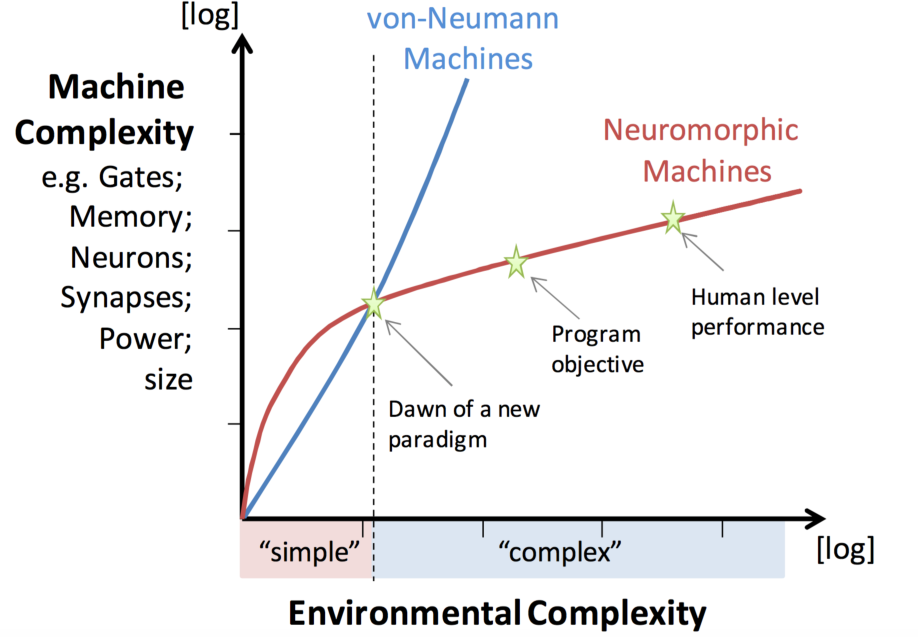
\includegraphics[height=3cm]{imgs/Synapse_plot_machine_vs_environmental_complexity.png}
        }
        \subfloat[\label{subfig:Marr_energy_eff_wall}]{%
            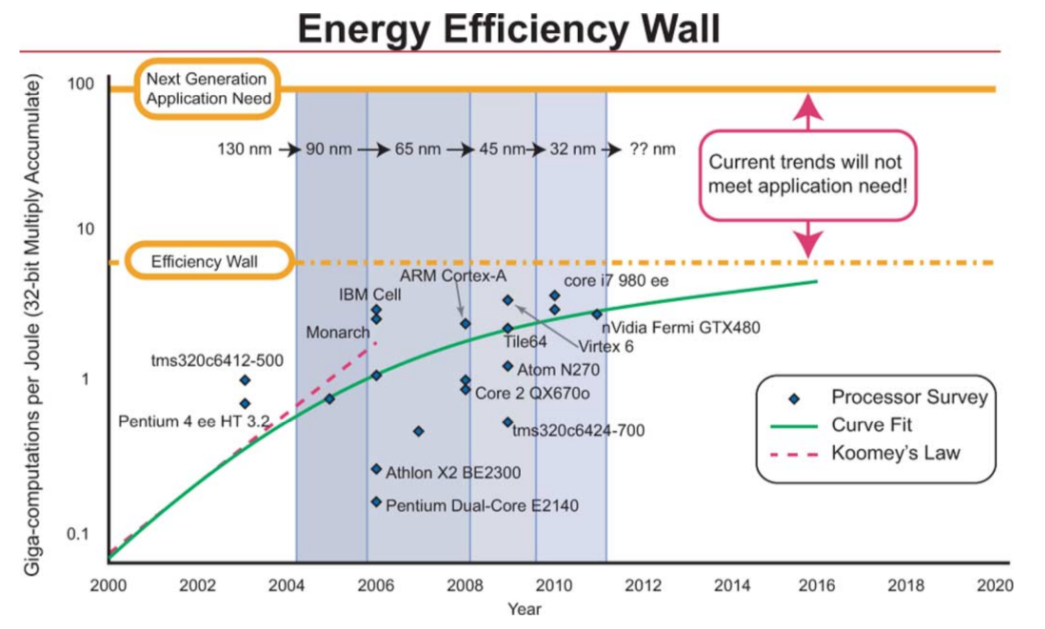
\includegraphics[height=3cm]{imgs/Marr_energy_eff_wall.png}
        }
    }
    \caption{Expected discrepancy between energy-efficiency requirements of future applications and the development of computing hardware.~\protect\subref{subfig:Synapse_plot_machine_vs_environmental_complexity} Image source: \citet{Farahini2016}, adapted from the \acs{DARPA} \acs{SyNAPSE} program.~\protect\subref{subfig:Marr_energy_eff_wall} Image source: \citet{Marr2013}.}
    \label{fig:energy_efficiency_issues}
\end{figure}
Although the neuromorphic prototypes of computing hardware such as \ac{SpiNNaker} \citep{Furber2014} or  IBM's TrueNorth \citep{Akopyan2015} dedicated to processing so-called \acp{SNN} are not technologically mature nor available as commercial products yet, they show promise to be a useful addition in future automotive applications.
Since these novel spiking-neuron architectures encapsulate a drastically different computing paradigm compared to the conventional von-Neumann architecture \citep{vonNeumann1993}, they also call for alternative algorithmic approaches and new programming substrates \citep{Amir2013}.

In this thesis, we investigate potential applications of neuromorphic approaches in automotive context.
Given the complexity of driving a car autonomously in all possible real-world situations, tackling the complete set of all necessary tasks is out of scope of a single thesis.
Therefore, we need to focus on certain sub-tasks.
Regarding this selection process, we contemplate two concepts.
We categorize tasks necessary for highly automated driving using the perception-action-cycle and rate their level of complexity using Moravec's paradox \citep{Moravec1988}.
Moracev's paradox postulates the observation, that tasks or skills that seem effortless to humans are harder to reverse-engineer than tasks we experience or expect to be difficult.
Moracev argues, that we learned those seemingly effortless skills over billions of years of evolution through experience about the nature of the world such that they became unconscious to us.
A good example of this paradox is the fact that artificial systems are already able to defeat the world's best human players in games like Chess \citep{Hsu2002} or Go \citep{Silver2016}, which are considered particularly difficult by humans.
On the other hand, we are still struggling to create robots that solve seemingly effortless sensorimotor tasks like climbing stairs or opening doors \citep{Guizzo2015, Norton2017}.

The perception-action-cycle \citep{Fuster2004} is the concept of a circular information flow between an organism or agent (living or artificial) when interacting with its environment through goal-directed behavior (cf. Fig. \ref{fig:perc-act-cicle}).
\begin{figure}[t!]
	\centering
	%	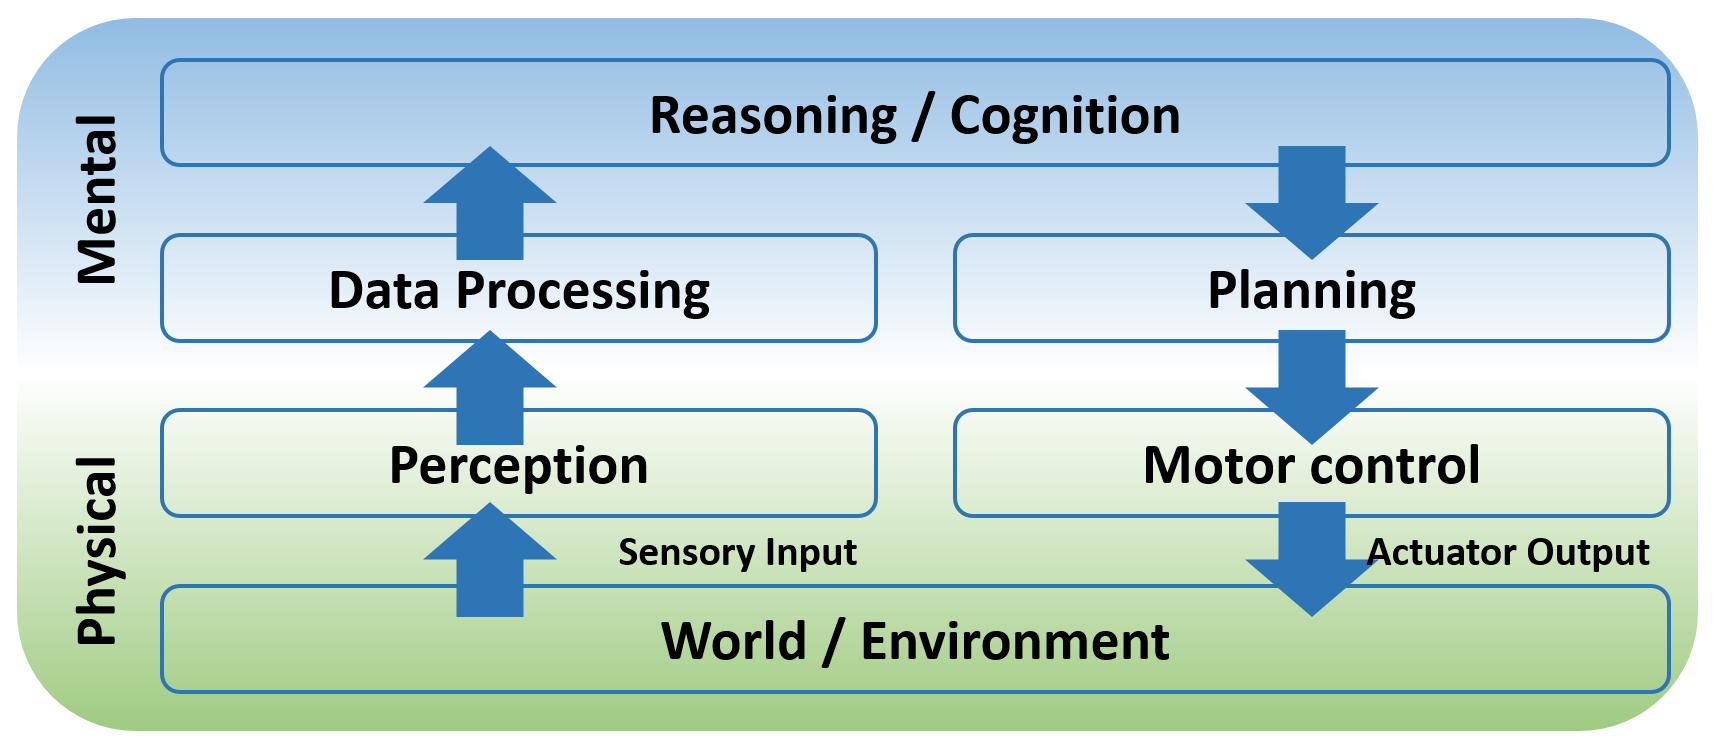
\includegraphics[width=0.85\textwidth, height=150px]{imgs/ActionPerceptionCycle.eps}
	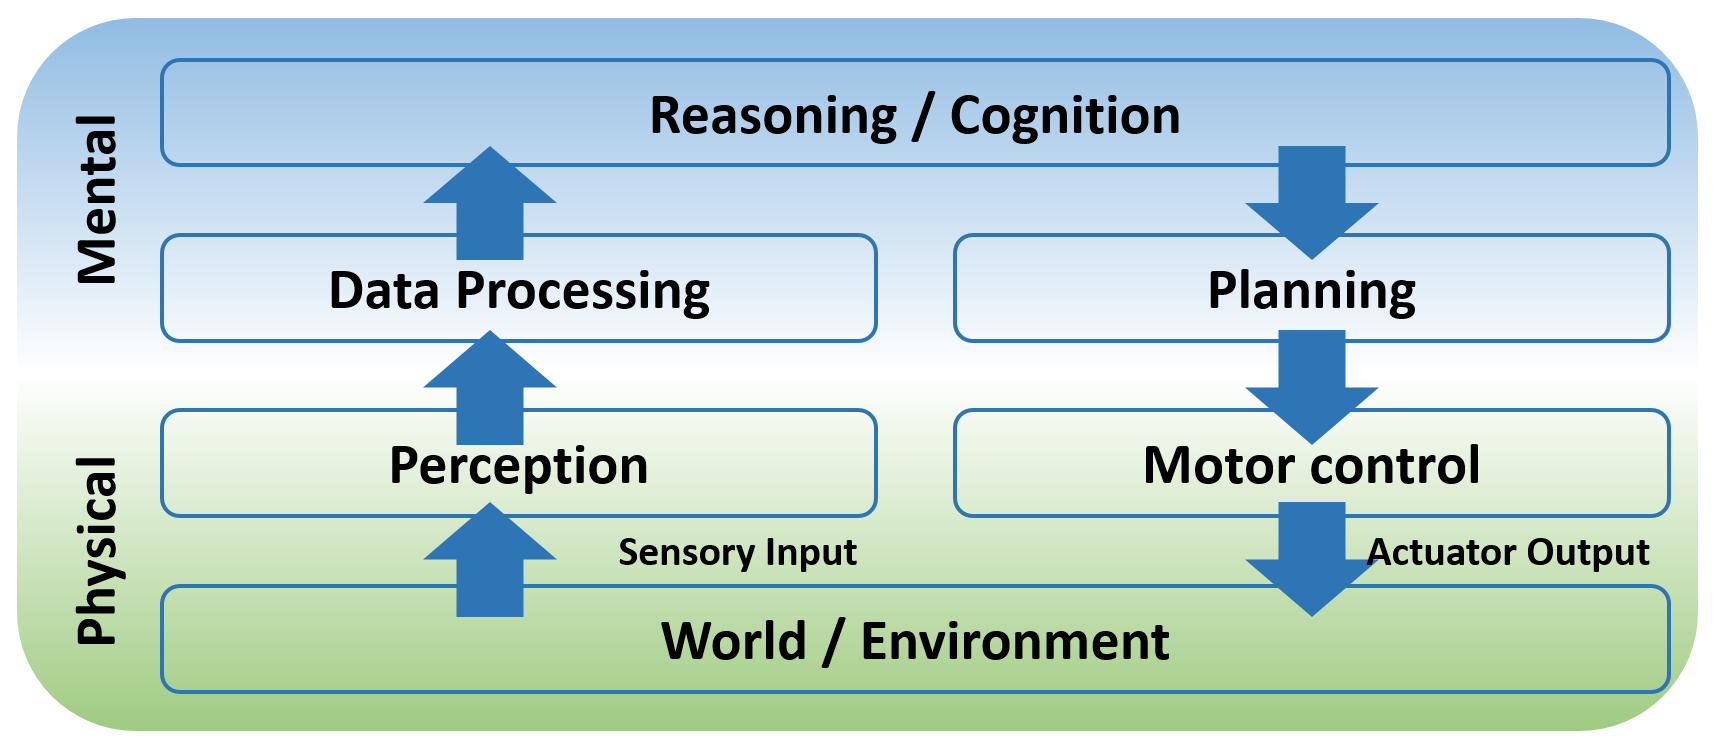
\includegraphics[width=0.85\textwidth]{imgs/ActionPerceptionCycle.eps}
	\caption{Schematic visualization of the perception-action-cycle}
	\label{fig:perc-act-cicle}
\end{figure}
Instead of considering the directional aspects of the cycle in the opposite categories of perception and action, it is also common to separate tasks in terms of hierarchy \citep{Loeb2014}.
Interaction with the physical world through sensing and manipulation is considered on a lower hierarchical level within the perception-action-cycle while formation of mental representations and reasoning about them reside on a higher level.
We refer to those different hierarchical levels as \emph{physical} and \emph{mental} or \emph{lower} and \emph{upper} interchangeably.

Considering the physical/lower level of the perception-action-cycle, \acp{DNN} have recently shown significant progress and success at perception tasks like object detection and classification.
Therefore, we believe a lot more research is necessary until neuromorphic approaches using \acp{SNN} are sufficiently mature to compete with those traditional approaches, although current work in this directions shows promising results \citep{Hunsberger2015}.
Similar arguments hold true for automated learning approaches regarding vehicle control.
Although sophisticated learning techniques show promise to improve motor control, to date most controllers for automated vehicles or robots in general are "designed and tuned by human engineers" \citep{Deisenroth2013}.
One of the main reasons is the fact that control of an automated vehicle is an extremely safety-critical domain, while at the same time machine learning approaches in general pose additional challenges regarding safety validation \citep{Koopman2016}.
Furthermore, those tasks on the physical level of the perception-action-cycle are solved effortlessly by humans and therefore, according to Moravec's paradox, we should expect them to be hard to master for artificial learning systems.
Therefore, we decided to focus on the mental/upper part of the perception-action-cycle in this thesis.
On the one hand, we believe that tasks in this part of the cycle show promise to benefit most from neuromorphic approaches.
On the other hand, "mental" tasks do not necessarily need to be performed and evaluated in closed-loop systems, which make them less problematic regarding safety issues, and therefore ideal candidates for further investigations.
It should be clear however, that "perception/action and higher level cognition are not two independent parts of one systems, but rather two integrated aspects of cognitive beings such as as ourselves" \citep{Eliasmith2013}.
Current artificial systems are still far away from integrating both aspect effectively and more research will be necessary to close this gap.

Precise knowledge about the current state of its environment is essential for any autonomous agent and biological organism alike to plan a secure path for navigation and to safely interact with the world.
In case of highly automated vehicles, perception of the outside world usually happens through a variety of different sensory systems like cameras, \acs{RADAR} and \acs{LIDAR} sensors \citep{Aeberhard2015}.
This observed information needs to be collected and combined into a central environment model, which is the (mental) basis for further reasoning and decisions.
One essential ingredient for such a model of the environment, or mental tasks in general, is knowledge or information representation.
It is an open research question to date, how the human brain represents knowledge and what underlying neural or computational substrate it uses to encode information \citep{Wang2003, Samsonovich2012, Handjaras2016}.
Most modern approaches to reasoning or cognitive tasks in context of robotics or automated driving are built upon Bayesian probability theory and use "computer-scientific" approaches to knowledge representation.
This could be lists of objects (cf. Fig. \ref{subfig:urban_object_lists}) with numerical encoding of properties when working on a higher level of abstraction.
On a lower level, another common approach especially in context of neural-network learning, is to label raw sensory data, for example individual pixels of images (cf. Fig. \ref{subfig:urban_semantic_labels}).
However, when we as humans observe a particular scene (e.g., while driving), our mental representation will probably be very different from those aforementioned approaches.
\begin{figure}[t!]
	\centering
	\subfloat[Urban traffic scenario\label{subfig:urban_scene}]{%
		\includegraphics[width=0.45\textwidth]{imgs/urban_scene.eps}
	}
	\subfloat[Pixel-wise labels\label{subfig:urban_semantic_labels}]{%
		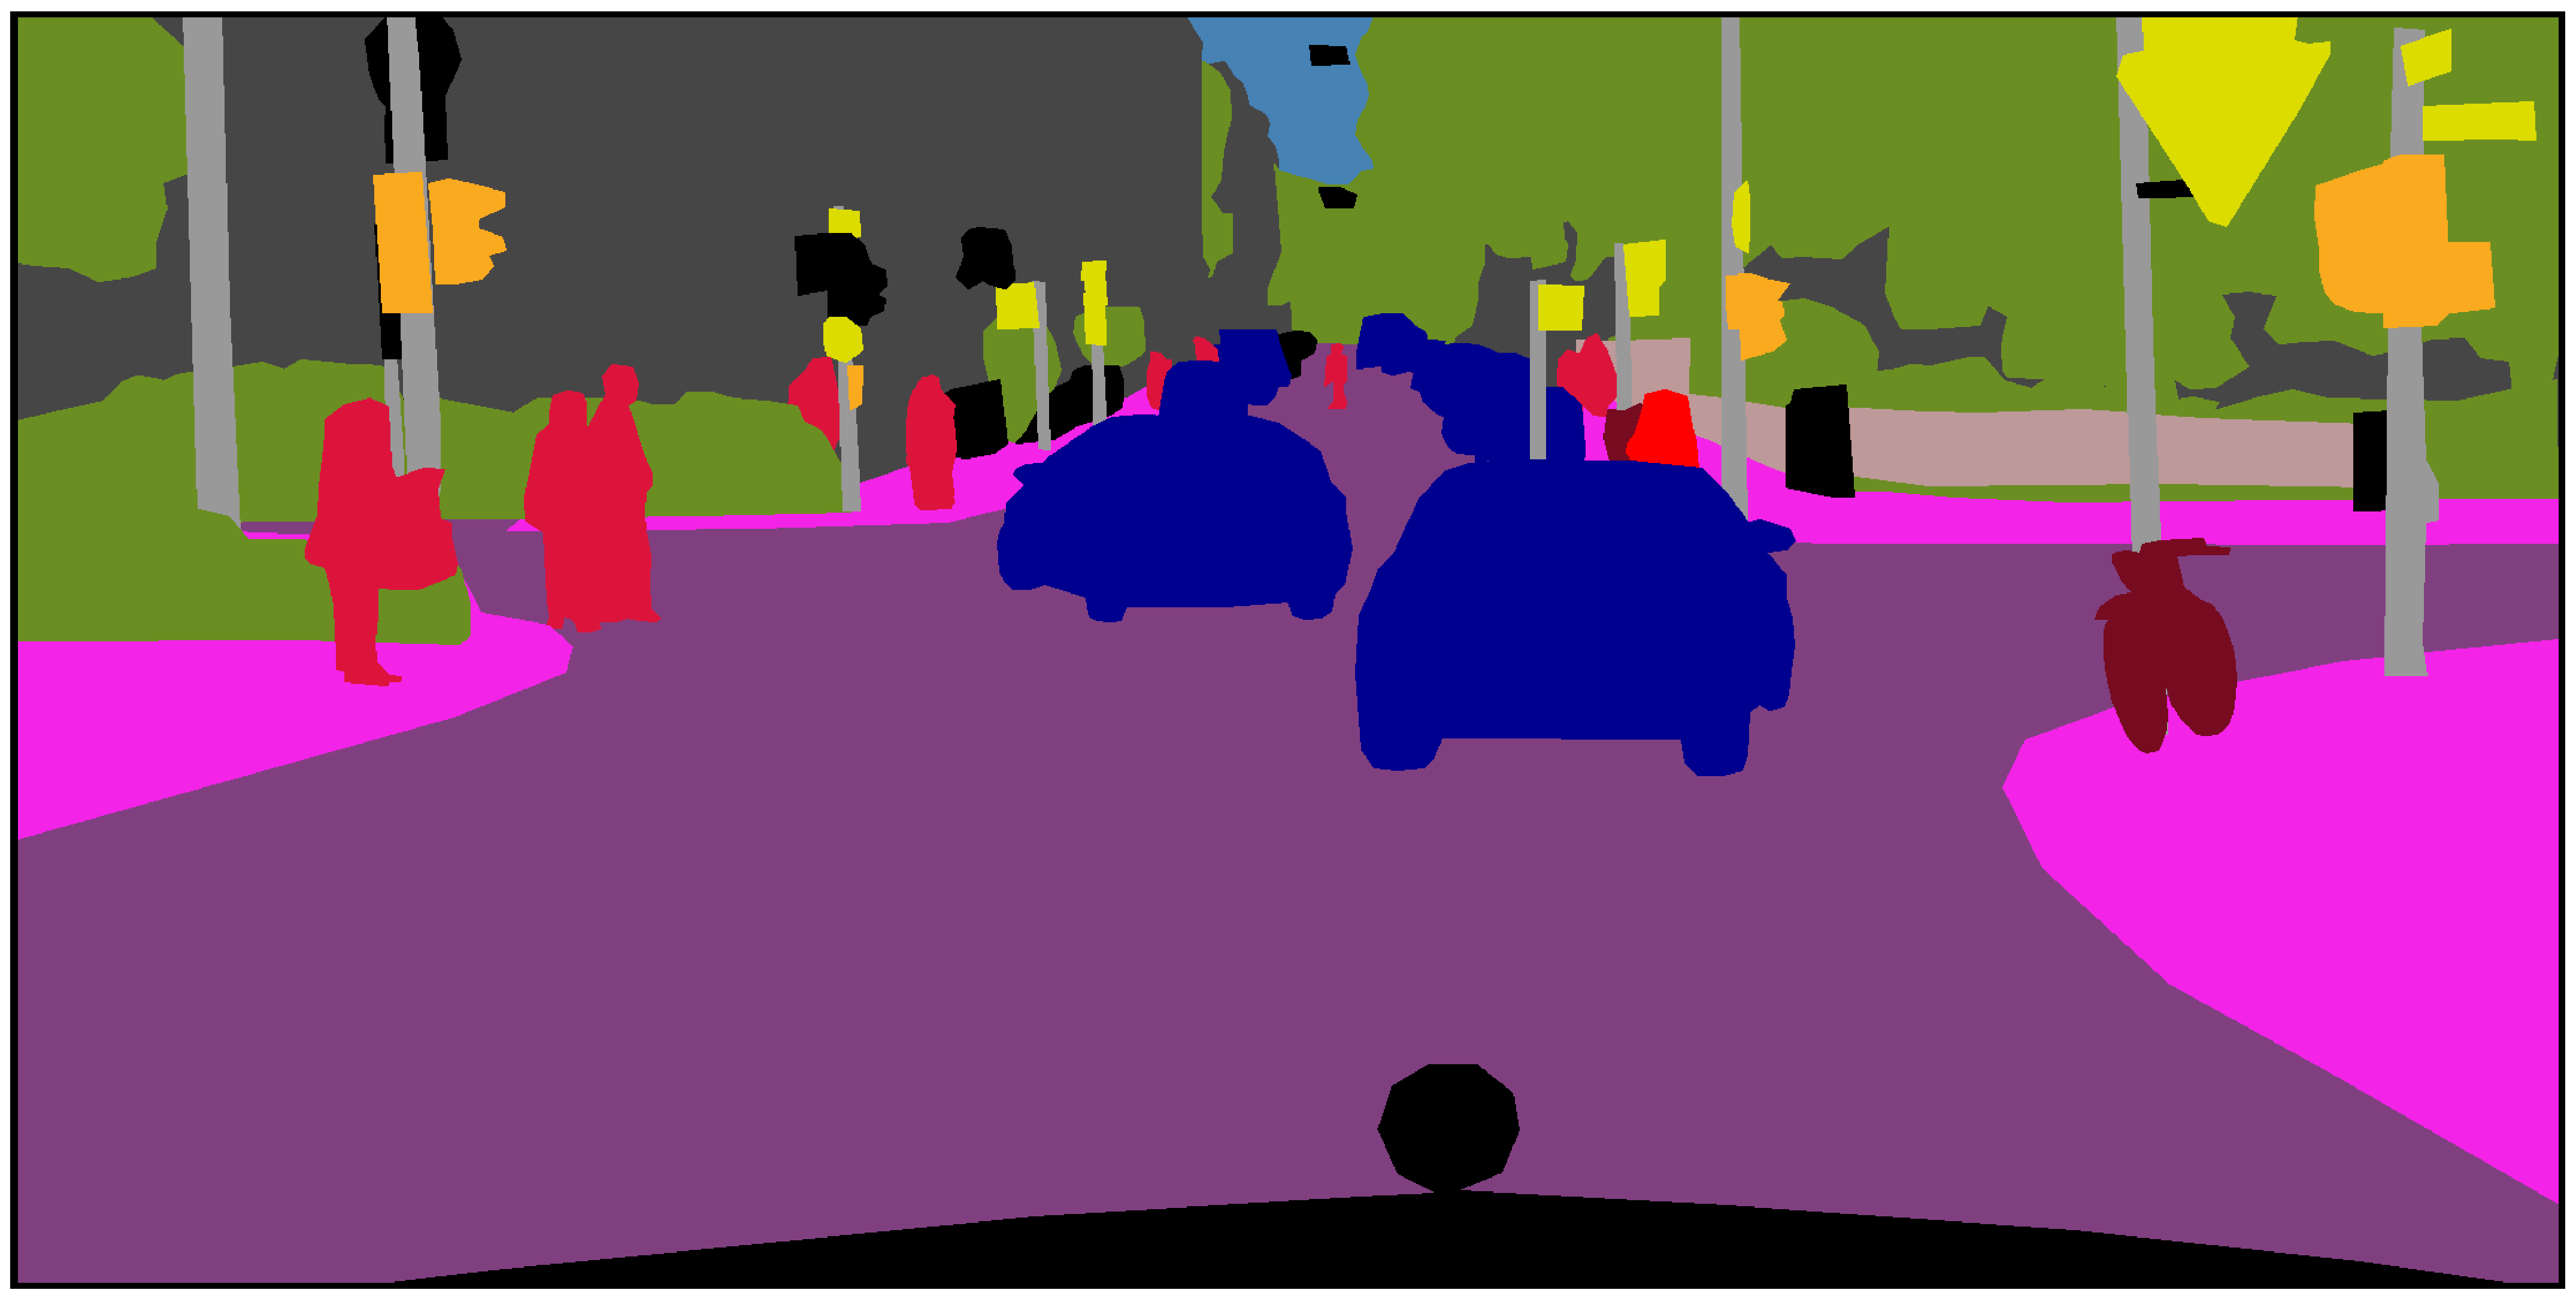
\includegraphics[width=0.45\textwidth]{imgs/urban_scene_pixel_labels.eps}
	}\\
	\subfloat[Bounding boxes indicating objects of interest\label{subfig:urban_scene_boxes}]{%
		\includegraphics[width=0.45\textwidth]{imgs/urban_scene_bound_boxes.eps}
	}
	\subfloat[Exemplary representation using lists of objects\label{subfig:urban_object_lists}]{%
		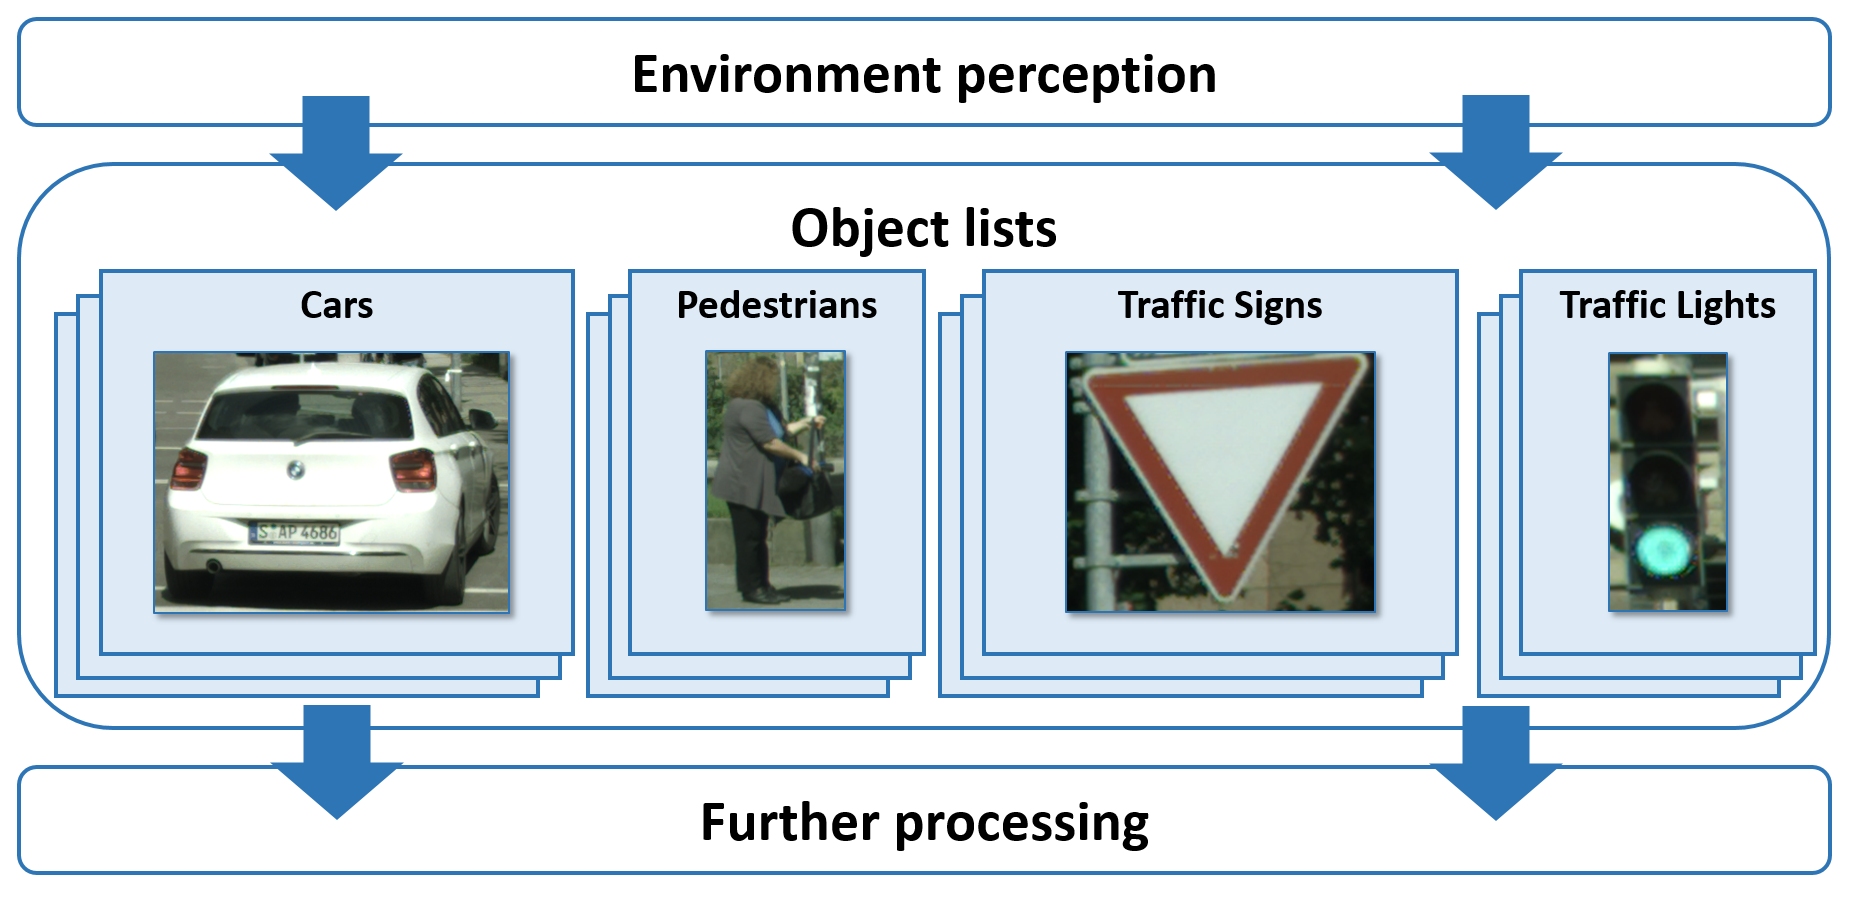
\includegraphics[width=0.45\textwidth, height=3.6cm]{imgs/urban_scene_object_lists.eps}
	}
	\caption{Example of urban driving scene with different approaches to representation. Images \ref{subfig:urban_scene}, \ref{subfig:urban_semantic_labels} and \ref{subfig:urban_scene_boxes} are (adapted) from the Cityscapes data set \citep{Cordts2016}.}
    \label{fig:urban_scene}
\end{figure}
A human observer's representation/description of Fig. \ref{subfig:urban_scene} would probably be in a semantic/linguistic form, for instance \emph{a blue car turning left, a white car turning right, three pedestrians waiting on the left side of the road, green traffic lights, a yield way sign}.
One common approach to encode such conceptual, semantic information or, more generally, natural language in computer-readable fashion is by using vector representations.
\acfp{VSA} is a term coined by \citet{Gayler2003} to cover this family of modeling approaches that represent symbols or structures by mapping them to (high-dimensional) vectors.

In this thesis, we present a first step towards a cognitive environment model for automotive applications using distributed representations.
We investigate the use of these vector representations for knowledge representation and reasoning in automotive context 
This approach to information encoding is rather generic and can be applied to various different tasks with little modifications to the representation itself.
Furthermore, \acp{VSA} offer to the opportunity to be implemented in a spiking neuron substrate \citep{Eliasmith2013}, which support efficient learning algorithms and deployment on dedicated neuromorphic hardware.
This allows us to combine the advantages of symbolization with the benefits of neural networks.
We investigate varying instantiations of our representation applied to different tasks.
In a first sample application we introduce a model learning to classify the current driving context based on a distributed representation of the current driving scene. 
The conceptual focus here is to capture semantics of the scene allowing conclusion about the type of environment the vehicle is currently navigating.
Another essential ingredient of an environment model especially in automotive context is precise knowledge about the current state and future development of all dynamic objects in the ego-vehicle's surroundings.
We focus on the task of predicting the behavior of those other traffic participants around the ego-vehicle based on a vector description of the current scene.
We hypothesize, that these structured representation have the potential to capture mutual interactions between dynamically moving agents.
Prediction of other traffic participants behavior also offers the opportunity to explore different learning approaches.
Human drivers have acquired comprehension through past experience of how other cars will probably act, but adapt this knowledge continuously when encountering new situations.
From this inspiration, we learn a generic model of dynamic behavior through offline (i.e., batch) training and refine this model when perceiving behavior of a particular object through online learning.
To complement the more high-level reasoning tasks with a perspective on neuromorphic control, a novel control architectures, that can be used to implement generic control algorithms in the language of \acp{SNN}.
This approach allows to divide larger tasks in small sub-networks combining the advantages of manual programming with neural network learning.

\section{Outline of the thesis}%
\label{sec:outline_of_the_thesis}

This section provides a brief overview of the thesis structure as well as a short summary for each chapter.
Chapter~\ref{chap:research_context} summarizes the state-of-the-art in several areas related to the core of the thesis at hand spanning from biologically inspired hardware and software over cognitive modeling techniques to automated driving research.
We give an overview over all of these sub-topics providing a detailed description where necessary while putting these details in context of a bigger picture.

Chapter~\ref{chap:introduction_to_vsas} introduces the key ingredients for the models developed in later chapter, distributed representations and \acp{SNN}, and establishes the mathematical apparatus and the essential theoretical properties of these ingredients.
Starting with proposing a more rigorous mathematical formalism to describe the general theory of \acp{VSA}, we proceed to the \ac{SPA} as a special case of \acp{VSA} with additional features and theory to be presented.
Furthermore, we give an introduction to the general ideas for cognitive modeling based on \acp{VSA} like vocabularies and structured representation generation.
Furthermore, we present a brief description of the \ac{NEF} and how it can be used to implement cognitive architectures based on vector representations in a spiking neuron substrate.

In chapter~\ref{chap:a_cognitive_approach_to_represent_automotive_scenes}, we proceed to present the general approach to encode automotive scenes in semantic vectors as representational substrate.
We show different approaches to generate vector vocabularies, which are the basic ingredients to built more complex, structured representations from them.
We demonstrate successful embedding of several similarity structures into vector vocabularies designed for automotive applications,
Additionally, we present several approaches to representing numerical values in our vector substrate introducing a novel approach based on a convolutive power, generalizing exponentiation to circular convolution.
We conclude the chapter with a thorough analysis regarding the systematic limitations regarding the vectors capacity, i.e., amount of information such vector representations can effectively store.

Chapter~\ref{chap:driving_context_classification} introduces the first sample instantiation of our vector representation applied to the task of driving context classification based on a scene vector encapsulating the current driving situation.
We establish the vector-based scene representation for the context classification task and use it as input data to a learning model implemented in a spiking neuron substrate.
To evaluate the model's performance, we present several reference learning systems using either the vector representation as well or visual input and compare them to human level performance.
Finally, we analyze the influence of the underlying vocabularies encoding different similarity structures on the learning model's classification performance.
All evaluations are conducted using real-world driving data.

In chapter~\ref{chap:behav_pred}, we introduce a second instantiation of scene representation to predict the behavior of other objects in the vehicle's surroundings.
In the context of vehicle trajectory prediction, we employ our novel approach to encode spatial information in distributed representations to encode the positions of several vehicles in vectors of fixed length.
We employ neural networks built from \ac{LSTM} units as well as simpler single-layer \acp{SNN} to predict vehicle trajectories based on past motion.
We analyze the influence of hyperparameters, information provided to the models as well as the composition of the training data on the models' prediction accuracy.
Furthermore, we compare the models with respect to situations in which one particular model outperforms the others.
Finally, we show that it is generally possible to detect abnormal samples indicating potentially dangerous situation based solely on the distributed vector representation and unsupervised learning.
The evaluation conducted in the chapter uses data from two different data sets containing real-world driving data.

Chapter~\ref{chap:mix_online_learning} introduces an extension of the proposed trajectory prediction models for online adaptation through incremental learning.
Building on the findings in chapter~\ref{chap:behav_pred}, we present a novel mixture of experts model implemented in a spiking neuron substrate and trained at run time to improve the prediction performance over several individual predictors.
Although trained at run time, one of the strengths of this model is that, instead of having to start from a completely blank state, it relies on several expert models, which have been previously trained and validated offline.
This model, as all models making predictions about the future, faces the issue that the actual motion of the predicted vehicle to compare the model's anticipated values to is future data and thus not available at the time the model actually makes its predictions.
To avoid potentially long delays in the online learning process, we propose a novel approach to spread the error signal of earlier predictions over later predictions.
Revisiting the data sets used in chapter~\ref{chap:behav_pred}, we evaluate two different variants of the mixture models adapting their weights either solely based on the prediction error or the current context of the scene.
We show, that our online learning model is able to improve over the individual predictors already after being exposed to a small set of example vehicles.

Chapter ~\ref{chap:closed_loop_neuromorphic_control_systems} presents a first step towards a neuromorphic control architecture by developing two sample instantiations of neurally-inspired control algorithms.
We establish neuromorphic control architectures, that can be used to implement generic control algorithms in the language of \acp{SNN} with the advantage, that the overall task can be divided into several sub-networks.
This approach gives the opportunity to combine manual programming with the advantages of neural network learning.
Manually programmed sub-tasks can either complement learning networks within the system or serve as an initial approximation of the desired function, which allows more directed learning to improve task performance avoiding the need to start learning from a completely blank state.
As mentioned earlier, control of an automated vehicle is an extremely safety-critical application.
Hence, we present two sample applications in simplified setup: one on mobile robot manipulation demonstrating initial manual programming of a non-trivial robotic task in a spiking neuron substrate and one on vehicle trajectory control demonstrating how manually programmed modules can be complemented by learning networks.

Chapter~\ref{chap:discussion} summarizes the work and interprets the results achieved in this thesis.
We discuss the main advantages of the representations and models proposed in this work while also addressing limitations indicated by either systematic or experimental analysis.
We conclude the thesis by proposing a series of extensions and improvements which potentially contribute to adopting the principles investigated in this thesis on a wider scale to obtain a more mature representation framework for automotive applications.

\section{Contributions of and to this thesis}%
\label{sec:contributions_of_and_to_this_thesis}

This thesis presents a first step towards a cognitive environment model for automated vehicles and thereby a provides a novel perspective to knowledge representation in automotive context.
The two key ingredients for our approach are distributed representations and \acp{SNN}, which in combination offer a promising modeling substrate for cognitive tasks as shown in \citet{Eliasmith2013, Eliasmith2012}. 
The possibility to implement distributed representations in a spiking neuron substrate offers an interesting possibility to combine symbol-like processing with the strength of neural network learning.
Additionally, \acp{SNN} are one option to tackle increasing energy-efficiency requirements in future automated vehicles equipped with a plethora of sensor and computing systems.
This thesis presents a strict mathematical formalism regarding the theory of distributed representations, summarizing their key features in a generic framework.
Thereby, we lay the foundation for our novel approach to build structured representations of automotive scenes.
We demonstrate the general feasibility of our approach in two sample instantiations.
For all the models and representation approaches investigated in this thesis, we present a thorough and detailed analysis regarding parameters and accuracy including a comparison to several baseline models.
While the models employing our structured representations achieve promising results in terms of accuracy without clearly outperforming more traditional approaches, we expect the critical benefits of our approach to reveal when deployed on specialized computing hardware. 
As shown by \citet{Hunsberger2016}, implementing learning models in \acp{SNN} is often a trade-off between energy-efficiency and accuracy.
Finally, we establish neuromorphic control architectures, that can be used to implement generic control algorithms in the language of \acp{SNN}.
This approach can benefit from splitting larger tasks in small sub-networks, that can be manually programmed to complement or bootstrap learning networks.

This dissertation was supported by the \ac{BMW} Group, where I was employed as doctoral candidate and later in a permanent position during the preparation of this thesis.
Therefore, parts of the literature review and text that presents the research context in chapter~\ref{chap:research_context}, especially the section on neuromorphic computing hardware, was conducted in collaboration with \ac{BMW} colleagues.
The research on the mobile manipulation task was conducted during a collaboration project between \ac{TUM} and University of Waterloo while the work on vehicle trajectory control was supported by Benjamin Zorn during his internship at \ac{BMW}.
The approaches, principles and models presented in the sections on structured vocabularies in chapters~\ref{chap:a_cognitive_approach_to_represent_automotive_scenes} and~\ref{chap:driving_context_classification} were developed in collaboration with Robert Darius during the preparation of his Master's thesis \citep{Darius2018} under my supervision at \ac{BMW} Group.
Many of the novel approaches presented in this thesis arose from discussions with researchers from the \ac{CNRG} at University of Waterloo, where I spent a six week research visit in summer 2017.
This research visit spawned a follow-up collaboration project between \ac{BMW} and \ac{CNRG}, during which parts of chapters~\ref{chap:behav_pred} and~\ref{chap:mix_online_learning} were developed in collaboration.
This collaboration covered mainly the implementation of the \ac{LSTM} model based on numerical input in chapter~\ref{chap:behav_pred} as well as discussions about the online learning approach presented in chapter~\ref{chap:mix_online_learning}.
Researchers involved in this collaboration co-authored some of the publications listed in~\ref{subsec:list_of_publications}.
Finally, figures displayed in this thesis, which have been reprinted or adapted from others or quotations are clearly marked as such.
Anything not indicated as quotation or external source is the author's original work.

\subsection{List of Publications}%
\label{subsec:list_of_publications}

The following list gives an overview of the publications written and submitted during the preparation and work on this thesis.
Beside accepted and published articles, we also list submitted but still pending manuscripts waiting for review or final publications at the time of submission of the thesis.

\subsubsection{Accepted peer-reviewed journal papers}
\begin{enumerate}
	\item \printpublication{Mirus2018a}
\end{enumerate}

\subsubsection{Accepted peer-reviewed conference papers}
\begin{enumerate}
	\item \printpublication{Mirus2019}
	\item \printpublication{Mirus2019a}
	\item \printpublication{Mirus2018}
\end{enumerate}

\subsubsection{Submitted peer-reviewed journal papers}
\begin{enumerate}
	\item \printpublication{Mirus2019b}
\end{enumerate}

\subsubsection{Submitted peer-reviewed conference papers}
\begin{enumerate}
    \item \printpublication{Mirus2019c}
\end{enumerate}
%\todo[inline]{change chapter filenames}
